\documentclass[a4paper, 11]{article}
\usepackage{setspace}
\usepackage{amsmath}
\usepackage{graphicx}
\usepackage{subfig}
\usepackage{float}
\usepackage{pdfpages}
\usepackage{adjustbox}
\usepackage{subcaption}
\usepackage{authblk}
\usepackage{booktabs}
\usepackage{natbib}
\usepackage{url} 
\doublespacing
\begin{document}
\title{\LARGE \textbf{ Assessing the Impact of Anthropogenic and Natural Stressors on Motile Diversity in Coral Reef Ecosystems} \\
\vspace*{20mm}}

\author{\textbf{Pu Zhao} \\Email: pu.zhao23@imperial.ac.uk \vspace*{4mm}}

\date{August 2024 \vspace*{30mm}}

\affil{\textbf{Imperial College London} \vspace*{10mm}}
% Title Page
    \begin{titlepage}
    \maketitle
      
    \begin{center}
      \textbf{
      Submitted for the MSc in Computational Methods in Ecology and Evolution} 

    \end{center}
    
    \end{titlepage}


\pagebreak
\newpage
\thispagestyle{empty} 
\mbox{} 

\begin{center}
  \textbf{Declaration}
\end{center}


\noindent{I declare that the raw data was provided by my supervisor, Emma Ransome, from Imperial College London. \\ \\ I declare that I was responsible for all data processing.\\ \\ I also declare that no mathematical models were developed by either me or my supervisor. \\ \\My supervisors, James Rosindell and Emma Ransome, along with Margaux Steyaert, a PhD student of Emma Ransome, provided me with technical Q\&A support and feedback in developing the analyses presented.}



\pagebreak

\textit{Total word count: 5208 words.}

\doublespacing

\begin{abstract}
Coral reef ecosystems are among the most diverse and productive environments on Earth, but they face significant threats from both anthropogenic and natural stressors. This study assesses the impact of these stressors on the diversity of motile organisms, such as fish and crustaceans, within coral reef ecosystems. Using data from 370 Autonomous Reef Monitoring Structures (ARMS) across 143 sites in 14 countries, we analyzed species diversity through the Shannon-Wiener diversity Index. Our analysis revealed a complex relationship between stressors and biodiversity. Anthropogenic stressors, notably fishing, demonstrated a significant positive correlation with motile diversity, suggesting that increased fishing pressure may reduce predator dominance, thereby enhancing overall species diversity. In contrast, natural environmental stressors exhibited a non-linear, U-shaped effect on motile diversity, where moderate levels of stress initially decreased diversity but later facilitated recovery. These results highlight the intricate dynamics within coral reef ecosystems, emphasizing the need for more detailed studies to fully understand the interplay between various stressors and biodiversity.
\end{abstract}

% Introduction
\section{Introduction}

Coral reef ecosystems are among the most diverse and productive ecosystems on Earth, providing habitat for approximately 25\% of known marine species \citep{hoegh2017coral}. Large motile species, such as fish and crustaceans, play essential roles in these ecosystems by contributing to nutrient cycling and maintaining ecological balance. However, coral reefs are increasingly threatened by both natural and anthropogenic factors. For example, large-scale coral bleaching events caused by climate change (particularly through the mechanisms of ocean warming and acidification), although corals have the ability to recover naturally, frequent and severe bleaching events greatly shorten their recovery time \citep{knowlton2001future, bostrom2020coral}. In addition, anthropogenic activities such as overfishing, coastal development, and pollution further exacerbate the stress on coral reef ecosystems. These activities not only degrade the physical structure of the reefs but also affect the abundance and diversity of reef-associated species \citep{hoegh2017coral}.


Furthermore, Andrello et al. (2022) mapped six human pressures on coral reefs, including fishing, water pollution (nitrogen and sediments), coastal population, industrial development, and tourism, using the latest quantitative data. Their study highlighted that fishing and water pollution are the most common pressures on coral reefs worldwide, overfishing leads to the depletion of key species that are crucial for reef health and resilience, while pollution from farming and untreated sewage encourages the growth of harmful algae, which adds more stress to the coral. \citep{andrello2022global}. Previous studies have shown that changes in benthic cover and anthropogenic stressors can significantly impact the biodiversity and abundance of coral reef species. For instance, reductions in live coral cover are often associated with declines in fish populations and shifts in community composition. Moreover, the interaction between benthic cover and motile species like spiny lobsters and sea urchins demonstrates that these organisms rely heavily on specific habitat features, such as coral cover and the presence of holes and crevices for shelter and foraging \citep{zapata2021diel}. This suggests that coral cover and anthropogenic stressors may have significant impacts on motiles and need to be adequately studied. 

To better understand these dynamics, it is essential to consider the measures of biodiversity used in ecological studies. The measurement of biodiversity is a critical component of ecological studies, providing insights into the health and resilience of ecosystems. As Jost (2006) emphasizes, traditional diversity indices, such as the Shannon-Wiener and Gini-Simpson indices, have been widely used to quantify species diversity \citep{jost2006entropy}. However, these indices alone do not provide a complete picture of an ecosystem's diversity. Hill numbers, introduced by Hill (1973), offer a more unified and intuitive approach by transforming classical diversity measures into effective numbers of species. 

This study evaluates the impact of anthropogenic stressors and natural environmental factors on the diversity of motile organisms in coral reef ecosystems. The diversity changes of motile organisms under different stress environments were analyzed. Our hypothesis is that anthropogenic stressors have a significant positive impact on the motile diversity of coral reef ecosystems, with the positive effect of fishing being the most pronounced. Additionally, marine environmental stressors exhibit a non-linear, U-shaped relationship with motile diversity, meaning that the impact of marine environmental factors on motile diversity is not always positive or negative. In coral reef systems, moderate natural disturbances (such as storms of moderate intensity) can prevent any single species from becoming overly dominant, thereby maintaining higher species diversity\citep{connell1978diversity}.


% Methods
\section{Materials and Methods}

This study employs a quantitative research method aimed at analyzing the impact of various factors on motile diversity within coral reef ecosystems. The study is designed as a retrospective analysis, utilizing existing datasets provided by the advisor. The research data encompasses multiple time points and information from different locations within coral reef ecosystems, providing a comprehensive basis for analysis.

\subsection{Data Collection}

\noindent\textbf{Species Data}

The species data used in this study comes from Ransome Emma. This experiment involved deploying 370 Autonomous Reef Monitoring Structures (ARMS) at 143 sites across 14 countries and 5 oceanic regions. These sites span different oceans and regions, primarily in parts of the Pacific and Indian Oceans, such as the Line Islands and Indonesia. The map shows the precise geographical locations of the ARMS facilities, marked with red dots on the world map (see figure 1)

\begin{figure}[htbp]
    \centering
    \adjustbox{max width=0.8\linewidth}{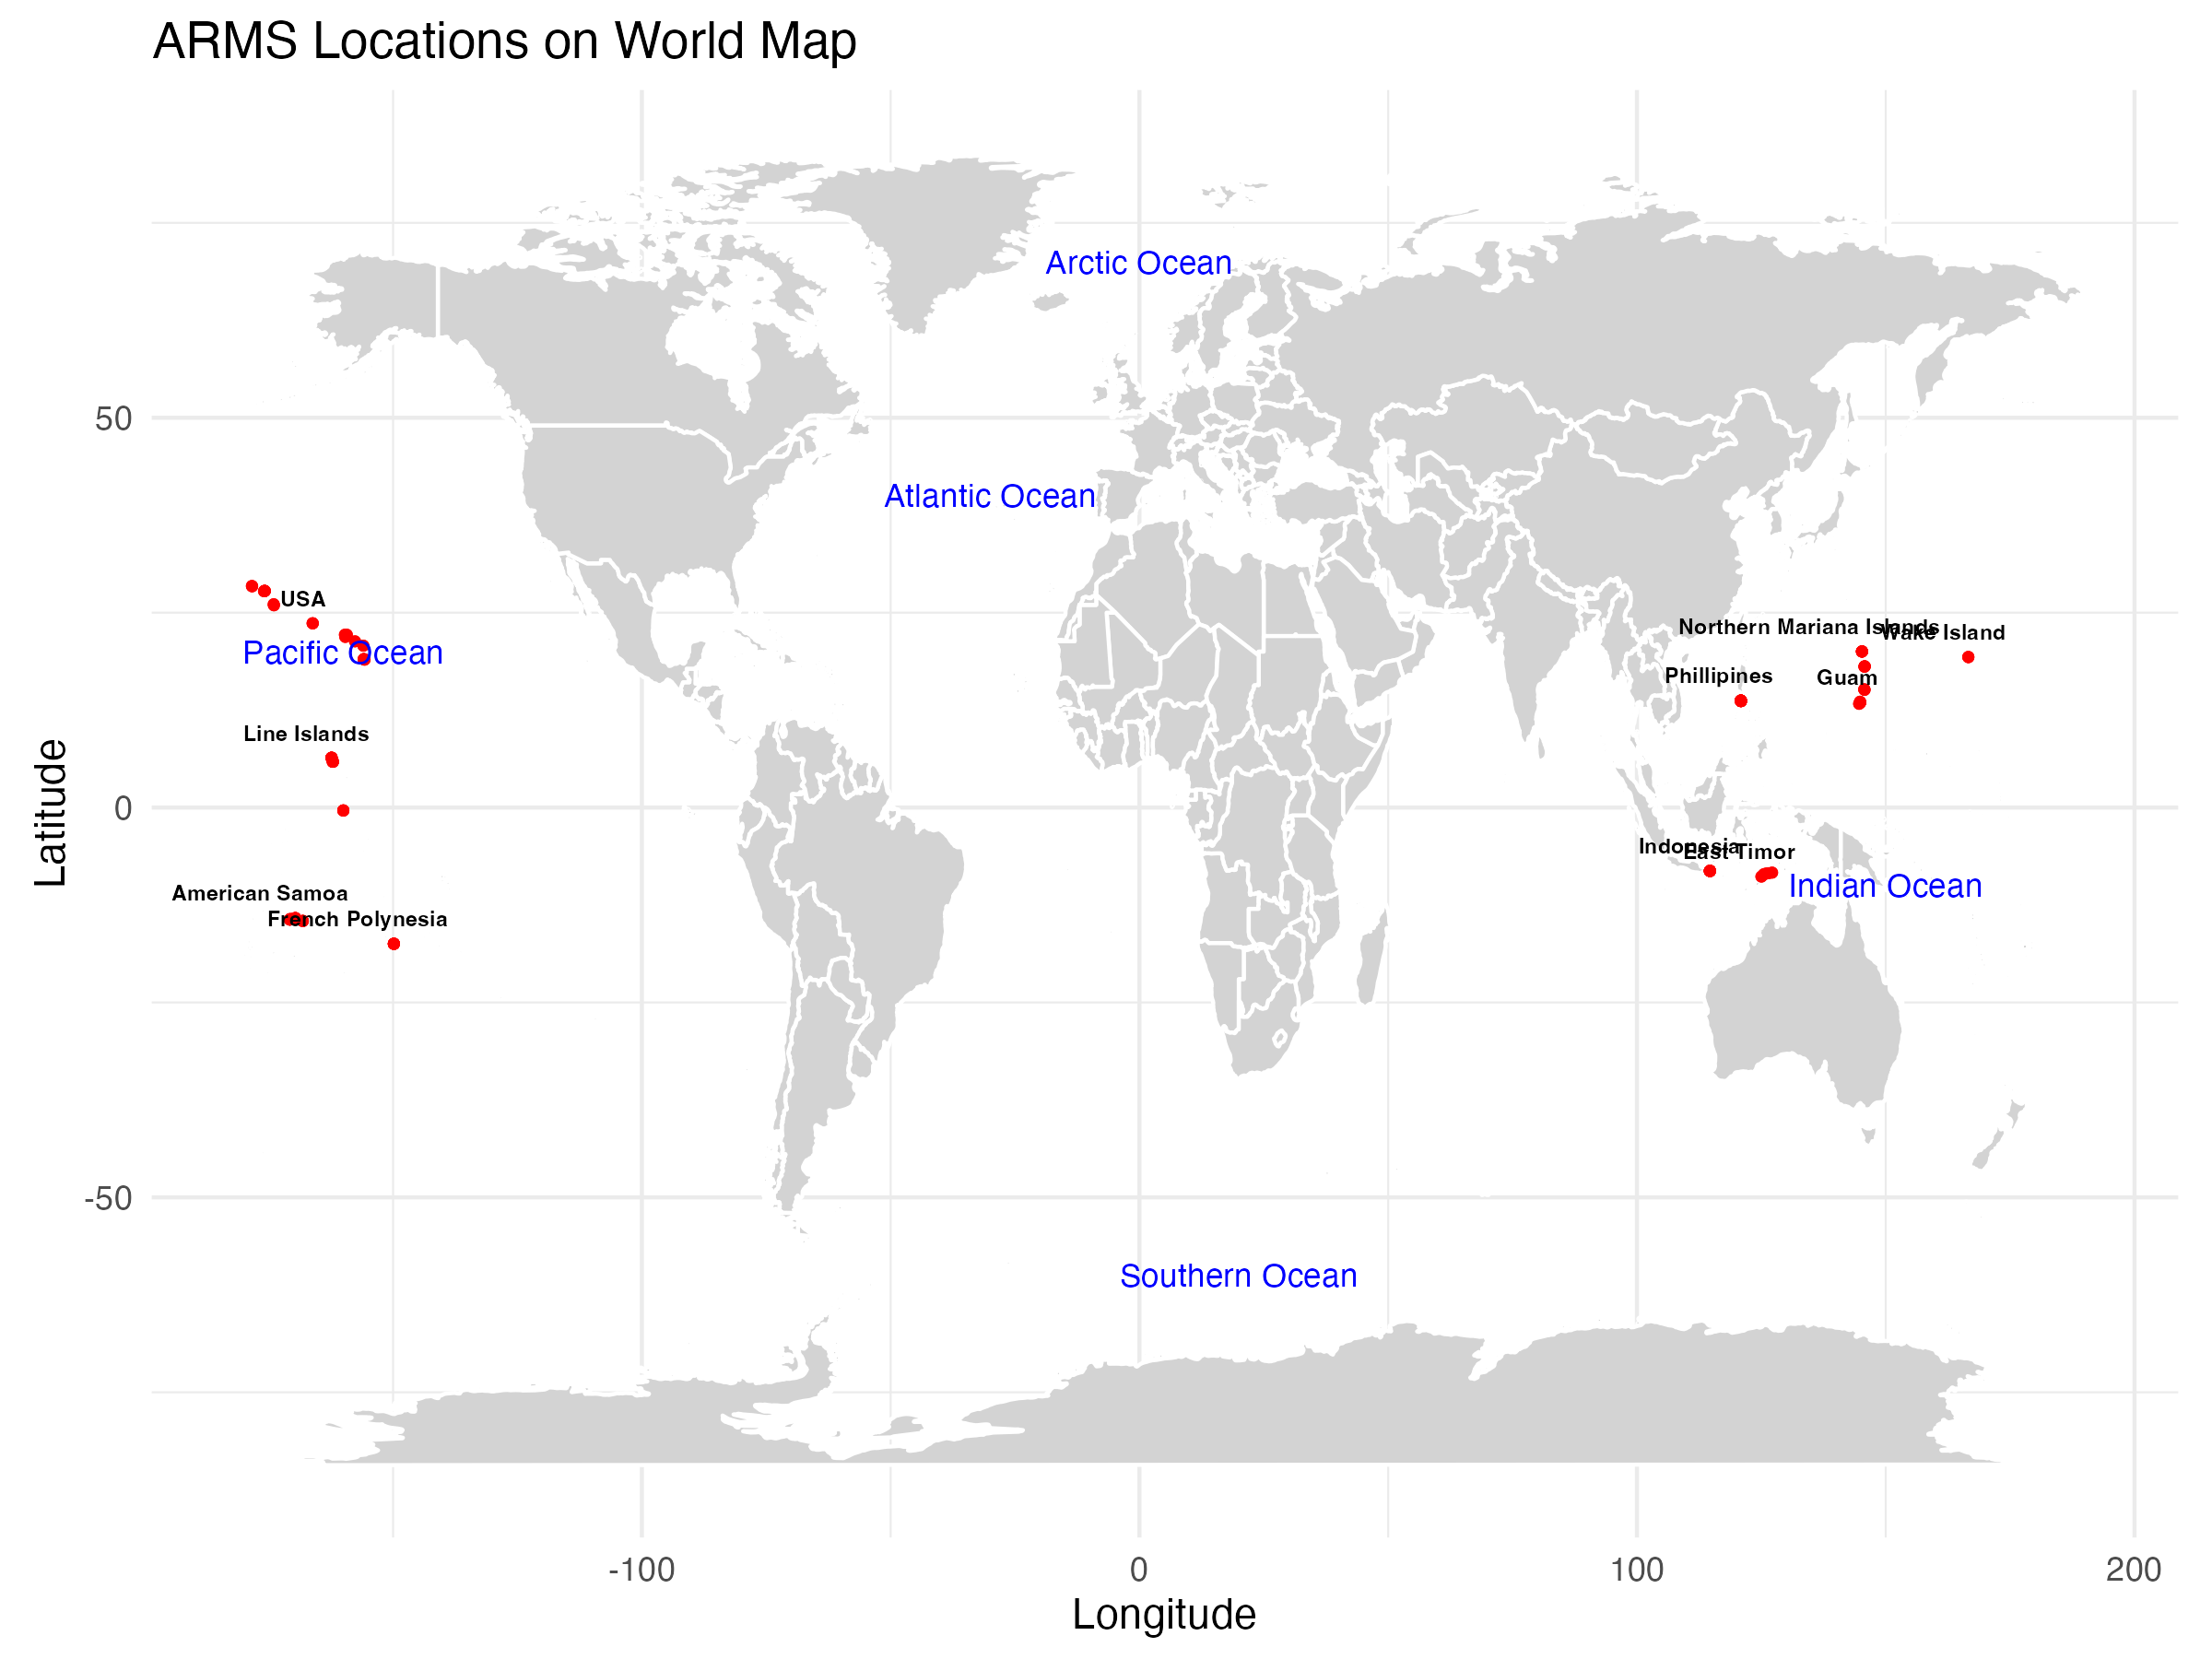
\includegraphics{../plot/Map.png}}
    \caption{Global distribution of ARMS locations. This figure shows the installation sites of the Autonomous Reef Monitoring Structures (ARMS) worldwide. These locations are marked with red dots. The figure was created using the R package [\textbf{\texttt{ggplot2}}] for data visualization and plotting, and [\textbf{\texttt{maps}}] for providing polygon data of the world map.}
\end{figure}

ARMS is a device used for monitoring and studying coral reef ecosystems, typically placed in different coral reef areas. These structures usually consist of multiple layers of plates, simulating the complex structure of coral reefs and attracting various marine organisms to settle. They are retrieved after one to three years, and the motile portion of the samples (100-500 micrometers and 500 micrometers-2 millimeters) was analyzed using 16S and COI markers. The sequencing data from these samples were processed using a custom bioinformatics pipeline (SimpleMetaPipeline). Subsequently, sequences in the samples' 16S rRNA gene that were clustered, with similarities above a certain threshold (usually 97\%), were classified as an Operational Taxonomic Unit (OTU). A total of 315,611 OTUs were integrated and classified into eight taxonomic levels:

  1. Rank\_1 (Root): Root node, representing the base level of the taxonomic tree.
  
  2. Rank\_2 (Domain/Kingdom): Such as Eukaryota.
  
  3. Rank\_3 (Phylum): Such as Arthropoda, Chordata, etc.
  
  4. Rank\_4 (Class): Such as Gastropoda, Malacostraca, etc.
  
  5. Rank\_5 (Order): Such as Decapoda, Nudibranchia, etc.
  
  6. Rank\_6 (Family): Such as Alpheidae, Dictyotaceae, etc.
  
  7. Rank\_7 (Genus): Such as Alpheus, Clathria, etc.
  
  8. Rank\_8 (Species/Subspecies): Such as Clytia simplex, Barentsia sp. HAW01, etc.\\


\noindent\textbf{Stress Data}

The marine environmental data for the ARMS used is sourced from Williamson et al. (2022) in their article "Monitoring shallow coral reef exposure to environmental stressors using satellite earth observation: the reef environmental stress exposure toolbox (RESET)." This study employs multiple satellite remote sensing data and the Google Earth Engine platform to develop the REEF Environmental Stress Exposure Toolbox (RESET) for monitoring shallow coral reef environmental stress exposure. The main environmental variables used in this study are:

1. Cloud Cover (cloud): Cloud cover can influence the amount of sunlight reaching the ocean surface, affecting the temperature and the photosynthetic activity of corals and algae. It also plays a role in mitigating thermal stress by blocking solar radiation. 

2. Current: Ocean currents refer to the continuous movement of seawater, driven by forces such as wind, temperature, and salinity differences. These currents play a crucial role in transporting nutrients, dispersing organisms, and influencing the temperature and salinity of the water around coral reefs, which can affect their health and resilience to stress. 

3. Depth: The depth of coral reefs influences light availability, water pressure, and temperature. Deeper reefs may be less exposed to temperature fluctuations, offering some protection against thermal stress.

4. Sea Surface Temperature (SST): SST is the water temperature close to the ocean's surface. It is a primary indicator of thermal conditions.

5. SST Variability: Sea Surface Temperature (SST) variability indicates fluctuations in the surface temperature of the ocean. High variability can stress coral reefs as it can cause periods of abnormal heat, which may lead to coral bleaching or other stress responses. 

6. Salinity: Salinity measures the concentration of salts in seawater. Changes in salinity levels can stress coral reefs, affecting their growth and survival.

7. Degree Heating Weeks (DHW): DHW is a measure of accumulated thermal stress on coral reefs.

8. SST Anomaly: SST anomaly represents deviations from the average SST, indicating unusual warming or cooling events. 

9. Wind: Wind affects the surface water movement and can influence upwelling.

These variables are standardized to SE scores ranging from 0 to 1 using the fuzzy logic method proposed by Williamson et al., quantifying each variable's environmental stress on coral reef ecosystems. In RESET, these SE scores collectively form a multivariable environmental stress exposure index, helping to assess the overall health of coral reefs and their ability to cope with environmental stressors \citep{williamson2022monitoring}.

The main anthropogenic stress factors used include six major non-climate stressors and cumulative scores, sourced from the global tropical coral reef anthropogenic stress dataset developed by Andrello et al. (2022). This dataset provides detailed information on 54,596 coral reef pixels worldwide (each pixel approximately 5 km × 5 km), covering six major non-climate stressors:
1. Fishing pressure. 
2. Sediment pollution.
3. Nitrogen pollution.
4. Coastal population pressure.
5. Industrial development pressure.
6. Tourism pressure.

To compare and evaluate the pressures faced by coral reefs, \citet{andrello2022global} converted the data for each of the six stressors for each coral reef pixel into global percentiles. This process ensures direct comparability between different stressors and reduces the impact of extreme values on the results. Subsequently, the cumulative pressure score (cumul\_score) is obtained by calculating the average percentile of the six stressors for each coral reef pixel. This cumulative score provides a quantitative evaluation of the comprehensive pressure levels faced by various coral reef regions \citep{andrello2022global}.\\


\noindent\textbf{Diversity indicators}

We use the Hill numbers as a diversity indicator in this research. Hill numbers adjust the sensitivity to the frequencies of different species through the parameter \( q \). Different values of \( q \) allow Hill numbers to account for the influence of both rare and common species. For instance, when \( q = 0 \), Hill numbers only consider species richness; when \( q = 1 \), it is the exponential form of the Shannon Index, balancing species abundance and evenness; when \( q = 2 \), it is the inverse of the Simpson Index, giving more weight to common species \cite{jost2006entropy}.

\begin{equation}
    {^q}D = \left( \sum_{i=1}^{S} p_i^q \right)^{\frac{1}{1-q}}
\end{equation}

where:
\begin{itemize}
    \item $q$ is the order of the Hill number,
    \item $S$ is the total number of species,
    \item $p_i$ is the relative abundance of species $i$.
\end{itemize}

The flexibility of the Hill number makes it the preferred tool for diversity analysis in ecological research. In calculating the Hill numbers for different ARMS, we chose to use the diversity function from the R package vegan instead of manual formula calculations to achieve simplicity and reduce the likelihood of errors. In addition, we mainly use \(q_1\) (Shannon-Wiener Index) as the diversity indicator for motile organisms in coral reef ecosystems. The Shannon Index simultaneously considers species richness and species evenness, providing a comprehensive diversity measure that reflects the number of species in a community and the distribution of their relative abundances. Compared to \(q_0\), which only considers the number of species, \(q_1\) better reflects the evenness of species distribution within the community. \(q_1\) has moderate sensitivity to both rare and dominant species, neither ignoring the presence of rare species nor overemphasizing the influence of common species. Therefore, it provides a more balanced perspective on diversity, avoiding the overestimation or underestimation of diversity in extreme cases. Compared to \(q_2\), which focuses more on dominant species, \(q_1\) captures more information about the internal structure of the community, especially when studying the evenness and overall diversity of community structure. In summary, choosing \(q_1\) as the diversity index strikes a balance between species richness and evenness, providing a more comprehensive and reliable evaluation of community diversity.

\subsection{Statistical Analyses}

In this research, the species data is presented as Operational Taxonomic Units (OTUs). Descriptive analysis was used to analyze the diversity distribution and basic characteristics of the species data. Subsequently, we averaged the overall environmental factor data (RESET\_score) for each ARMS and then combined it with anthropogenic pressure data. The reason for this approach is that RESET data contains a significant amount of temporal variation, with each sample obtaining a RESET score each month, whereas anthropogenic pressure data is fixed and does not vary over time. This step simplifies the subsequent regression analysis. 

For the combined data, we employed several regression models to evaluate the relative impact of various factors on motile diversity (\( q1 \)). The models included Linear Regression (LM), Polynomial Regression, and Random Forest. Linear Regression Model is a basic statistical method used to model the relationship between two or more variables \citep{montgomery2021introduction}. We used multiple linear regression to predict the impact of the combined RESET\_score and anthropogenic stressor score (cumul\_score) on \( q1 \). However, the influence of RESET\_score on \( q1 \) was not significant in the linear model, prompting us to explore Polynomial Regression to capture potential nonlinear relationships. Polynomial regression is an extended form of linear regression. It is used to model the nonlinear relationship between the dependent variable and one or more independent variables. Compared with simple linear regression, the power of the independent variables in the model increases, allowing the model to capture more complex nonlinear relationships \citep{seber2012linear}.

Additionally, the species data exhibited a nested structure, with different ARMS deployed across various locations, time points, and coral reef regions. Using Mixed-Effects Models allowed us to incorporate random effects to account for this nesting, thereby improving the accuracy and reliability of the models. Finally, we utilized Random Forest to analyze the importance of individual anthropogenic stressors, determining the extent of their impact on \( q1 \). Random Forest is an ensemble learning method that improves the prediction accuracy of the model by integrating multiple decision trees. Feature importance analysis is a very important step to understand which features contribute most to the prediction results of the model. Feature importance is determined by evaluating the average impact of each feature in all decision trees \citep{breiman2001random}.\\

\section{Results}

\begin{table}[H]
\centering
\begin{tabular}{lcccc}
\toprule
 & Estimate & Std. Error & t value & Pr($>|t|$) \\
\midrule
(Intercept) & 76.61 & 10.10 & 7.586 & 1.17e-12 *** \\
RESET\_score\_mean & -19.27 & 59.10 & -0.326 & 0.7448 \\
cumul\_score & 32.99 & 13.50 & 2.44 & 0.0154 * \\
\bottomrule
\end{tabular}
\caption{Coefficients for the model: lm(formula = q1 ~ RESET\_score\_mean + cumul\_score) \\
The coefficients display the estimates, standard errors, t-values, and p-values of the intercept and two independent variables.}
\label{tab:model1}
\end{table}

\vspace{1\baselineskip}

% Second Table
\begin{table}[H]
\centering
\begin{tabular}{lcccc}
\toprule
 & Estimate & Std. Error & t value & Pr($>|t|$) \\
\midrule
(Intercept) & 87.485 & 3.604 & 24.273 & $<$2e-16 *** \\
poly(RESET\_score\_mean, 1) & 66.102 & 51.730 & 1.278 & 0.2028 \\
poly(RESET\_score\_mean, 2) & 113.831 & 51.730 & 2.200 & 0.0289 * \\
\bottomrule
\end{tabular}
\caption{   Coefficients for the model: lm(formula = q1 ~ poly(RESET\_score\_mean, 2))\\ 
The coefficients display the estimates, standard errors, t-values, and p-values of the intercept and polynomial terms.}
\label{tab:model2}
\end{table}




In the multiple linear regression model (table 1), the p-value of the intercept is highly significant (p $<$ 0.005). Moreover, the estimated coefficient for \texttt{cumul\_score} is 32.99, with a p-value of 0.0154, which is less than 0.05, indicating that the effect of \texttt{cumul\_score} on \texttt{q1}[diversity] is statistically significant. This means that for every unit increase in \texttt{cumul\_score}, \texttt{q1} increases by an average of 32.99, showing a positive correlation between \texttt{cumul\_score} and \texttt{q1}. However, the p-value for \texttt{RESET\_score\_mean} is 0.7448, which is greater than 0.05, with an estimated coefficient of -19.27, indicating that the effect of \texttt{RESET\_score\_mean} on \texttt{q1} is not statistically significant, and suggesting that \texttt{RESET\_score\_mean} does not have a noticeable linear impact on \texttt{q1}. 
To further investigate the effect of the marine environmental factor \texttt{RESET\_score} on the motile diversity in the coral reef ecosystem, this study employed the polynomial regression model to explore the nonlinear relationship between \texttt{RESET\_score} and \texttt{q1}. Based on the results of the polynomial linear regression model (see table 2), we surprisingly found that the effect of \texttt{RESET\_score\_mean} on \texttt{q1} presents a significant quadratic relationship. The model results show that the estimated coefficient for the quadratic term of \texttt{RESET\_score} is 113.831, with a significant p-value of 0.0289.


\begin{figure}[H]
    \centering
    \adjustbox{max width=\linewidth}{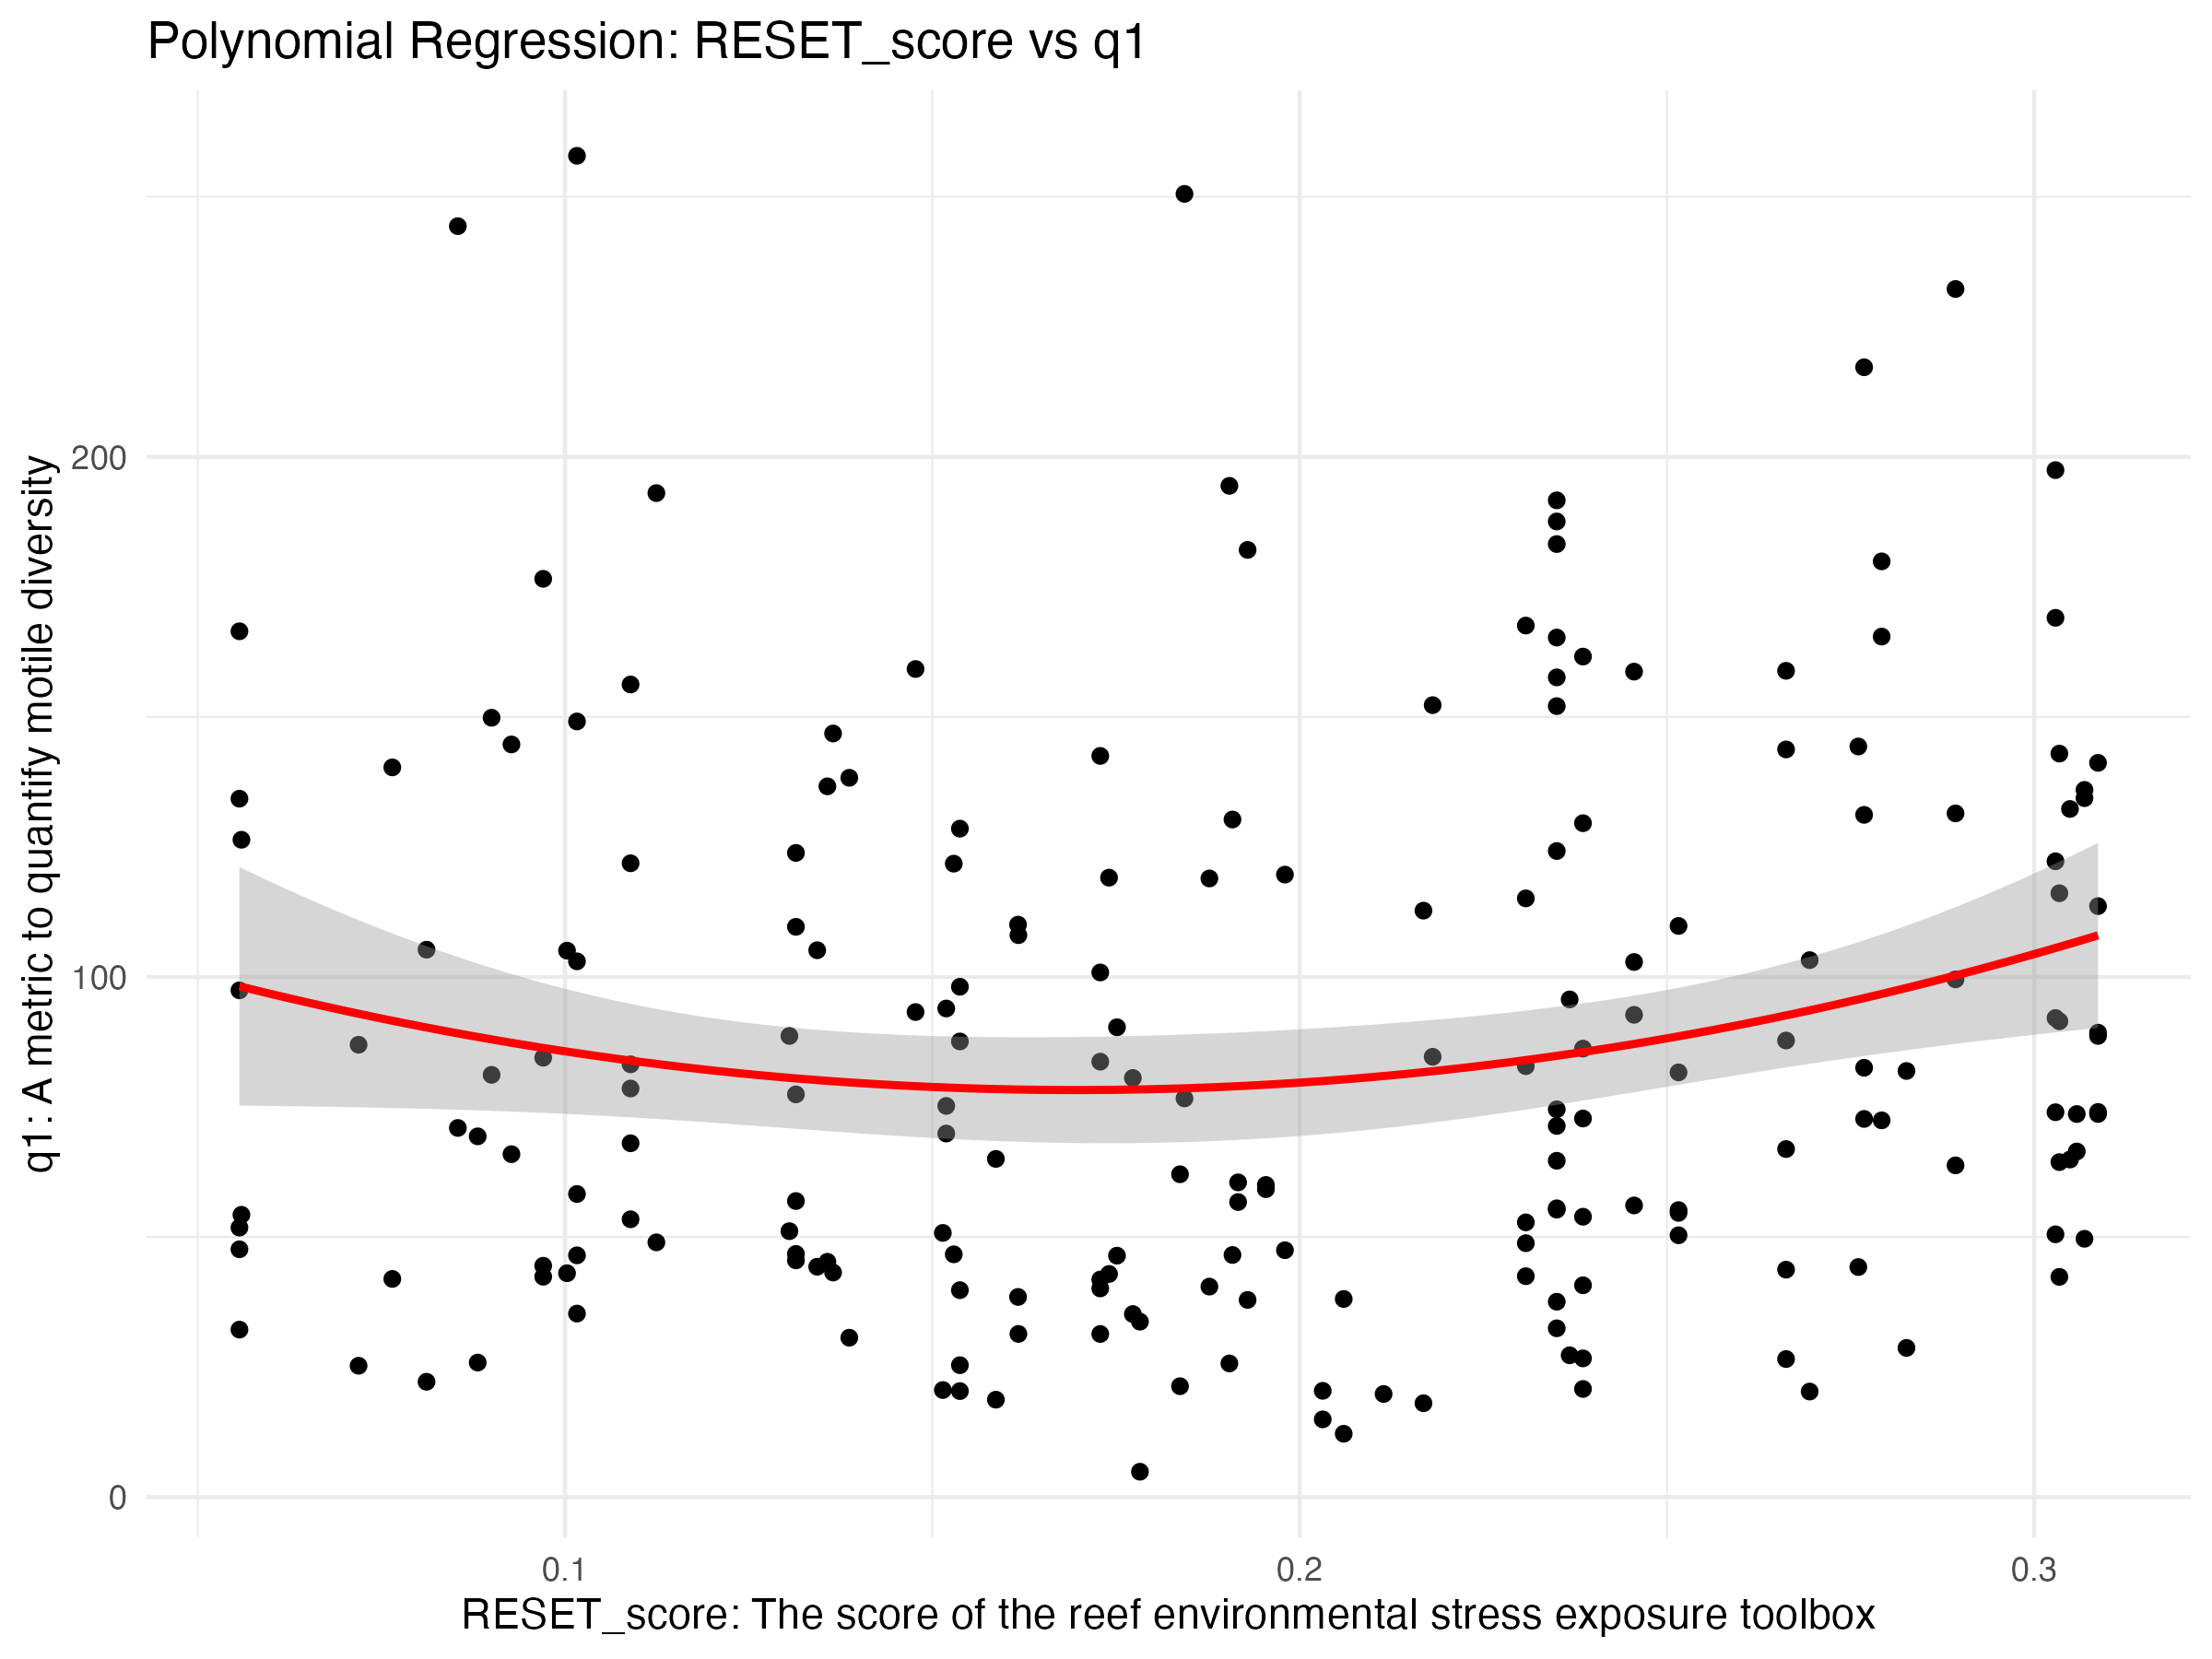
\includegraphics{../plot/reset_q1_poly.png}}
    \caption{Polynomial Regression: \texttt{RESET\_score\_mean} vs \texttt{q1}. This graph shows a scatter plot of the independent variable \texttt{RESET\_score\_mean} versus the dependent variable \texttt{q1}, along with a quadratic polynomial regression fit line. Each point represents an observation, the red curve indicates the quadratic polynomial regression fit, and the grey shaded area represents the confidence interval.}
\end{figure}

From the quadratic model, q1 exhibits a "U"-shaped relationship with RESET score (see Figure 2). Specifically, as the natural environmental pressure increases from a low level, q1 [diversity] decreases whist at higher levels of environmental pressure, q1 diversity increases with increasing pressure. The red line in polynomial regression analysis shows a trend of first descending and then ascending, which indicate that with the continuous increase in marine environmental pressure, the diversity of motile organisms in the coral reef system initially decreases and then increases. The range of environmental pressure scores in the figure is 0 to 0.35, corresponding to primary to moderate pressure.


\begin{table}[H]
\centering
\begin{tabular}{lcccc}
\toprule
 & Estimate & Std. Error & t value & Pr($>|t|$) \\
\midrule
(Intercept) & 122.472 & 68.972 & 1.776 & 0.0792 . \\
DHW & 214.451 & 199.326 & 1.076 & 0.2849 \\
SST & 14.169 & 54.334 & 0.261 & 0.7949 \\
‘SST anomaly‘ & -180.827 & 136.814 & -1.322 & 0.1897 \\
‘SST variability‘ & -658.872 & 1070.515 & -0.615 & 0.5398 \\
cloud & 13.719 & 250.426 & 0.055 & 0.9564 \\
current & 10.054 & 50.844 & 0.198 & 0.8437 \\
depth & -24.177 & 28.744 & -0.841 & 0.4025 \\
salinity & 5.144 & 127.140 & 0.040 & 0.9678 \\
wind & 23.635 & 208.155 & 0.114 & 0.9099 \\
\bottomrule
\end{tabular}
\caption{Coefficients for the model: lm(formula = q1 ~ DHW + SST + SST anomaly + SST variability + cloud + current + depth + salinity + wind)\\
The coefficients show the estimates, standard errors, t-values, and p-values for the intercept and 9 independent variables. The 9 independent variables correspond to 9 environmental factors in the marine natural environment.}
\label{tab:model_coefficients}
\end{table}

From the multiple linear regression model (table 3), we found that the influence of all individual marine environmental factors on the diversity index \(q_1\) is not significant within the linear model, as there is no evidence to prove that any single marine environmental factor is linearly correlated with \(q_1\) (all variables have \(p\) values $>$ 0.05). 


\begin{figure}[H]
    \centering
    \adjustbox{max width=\linewidth}{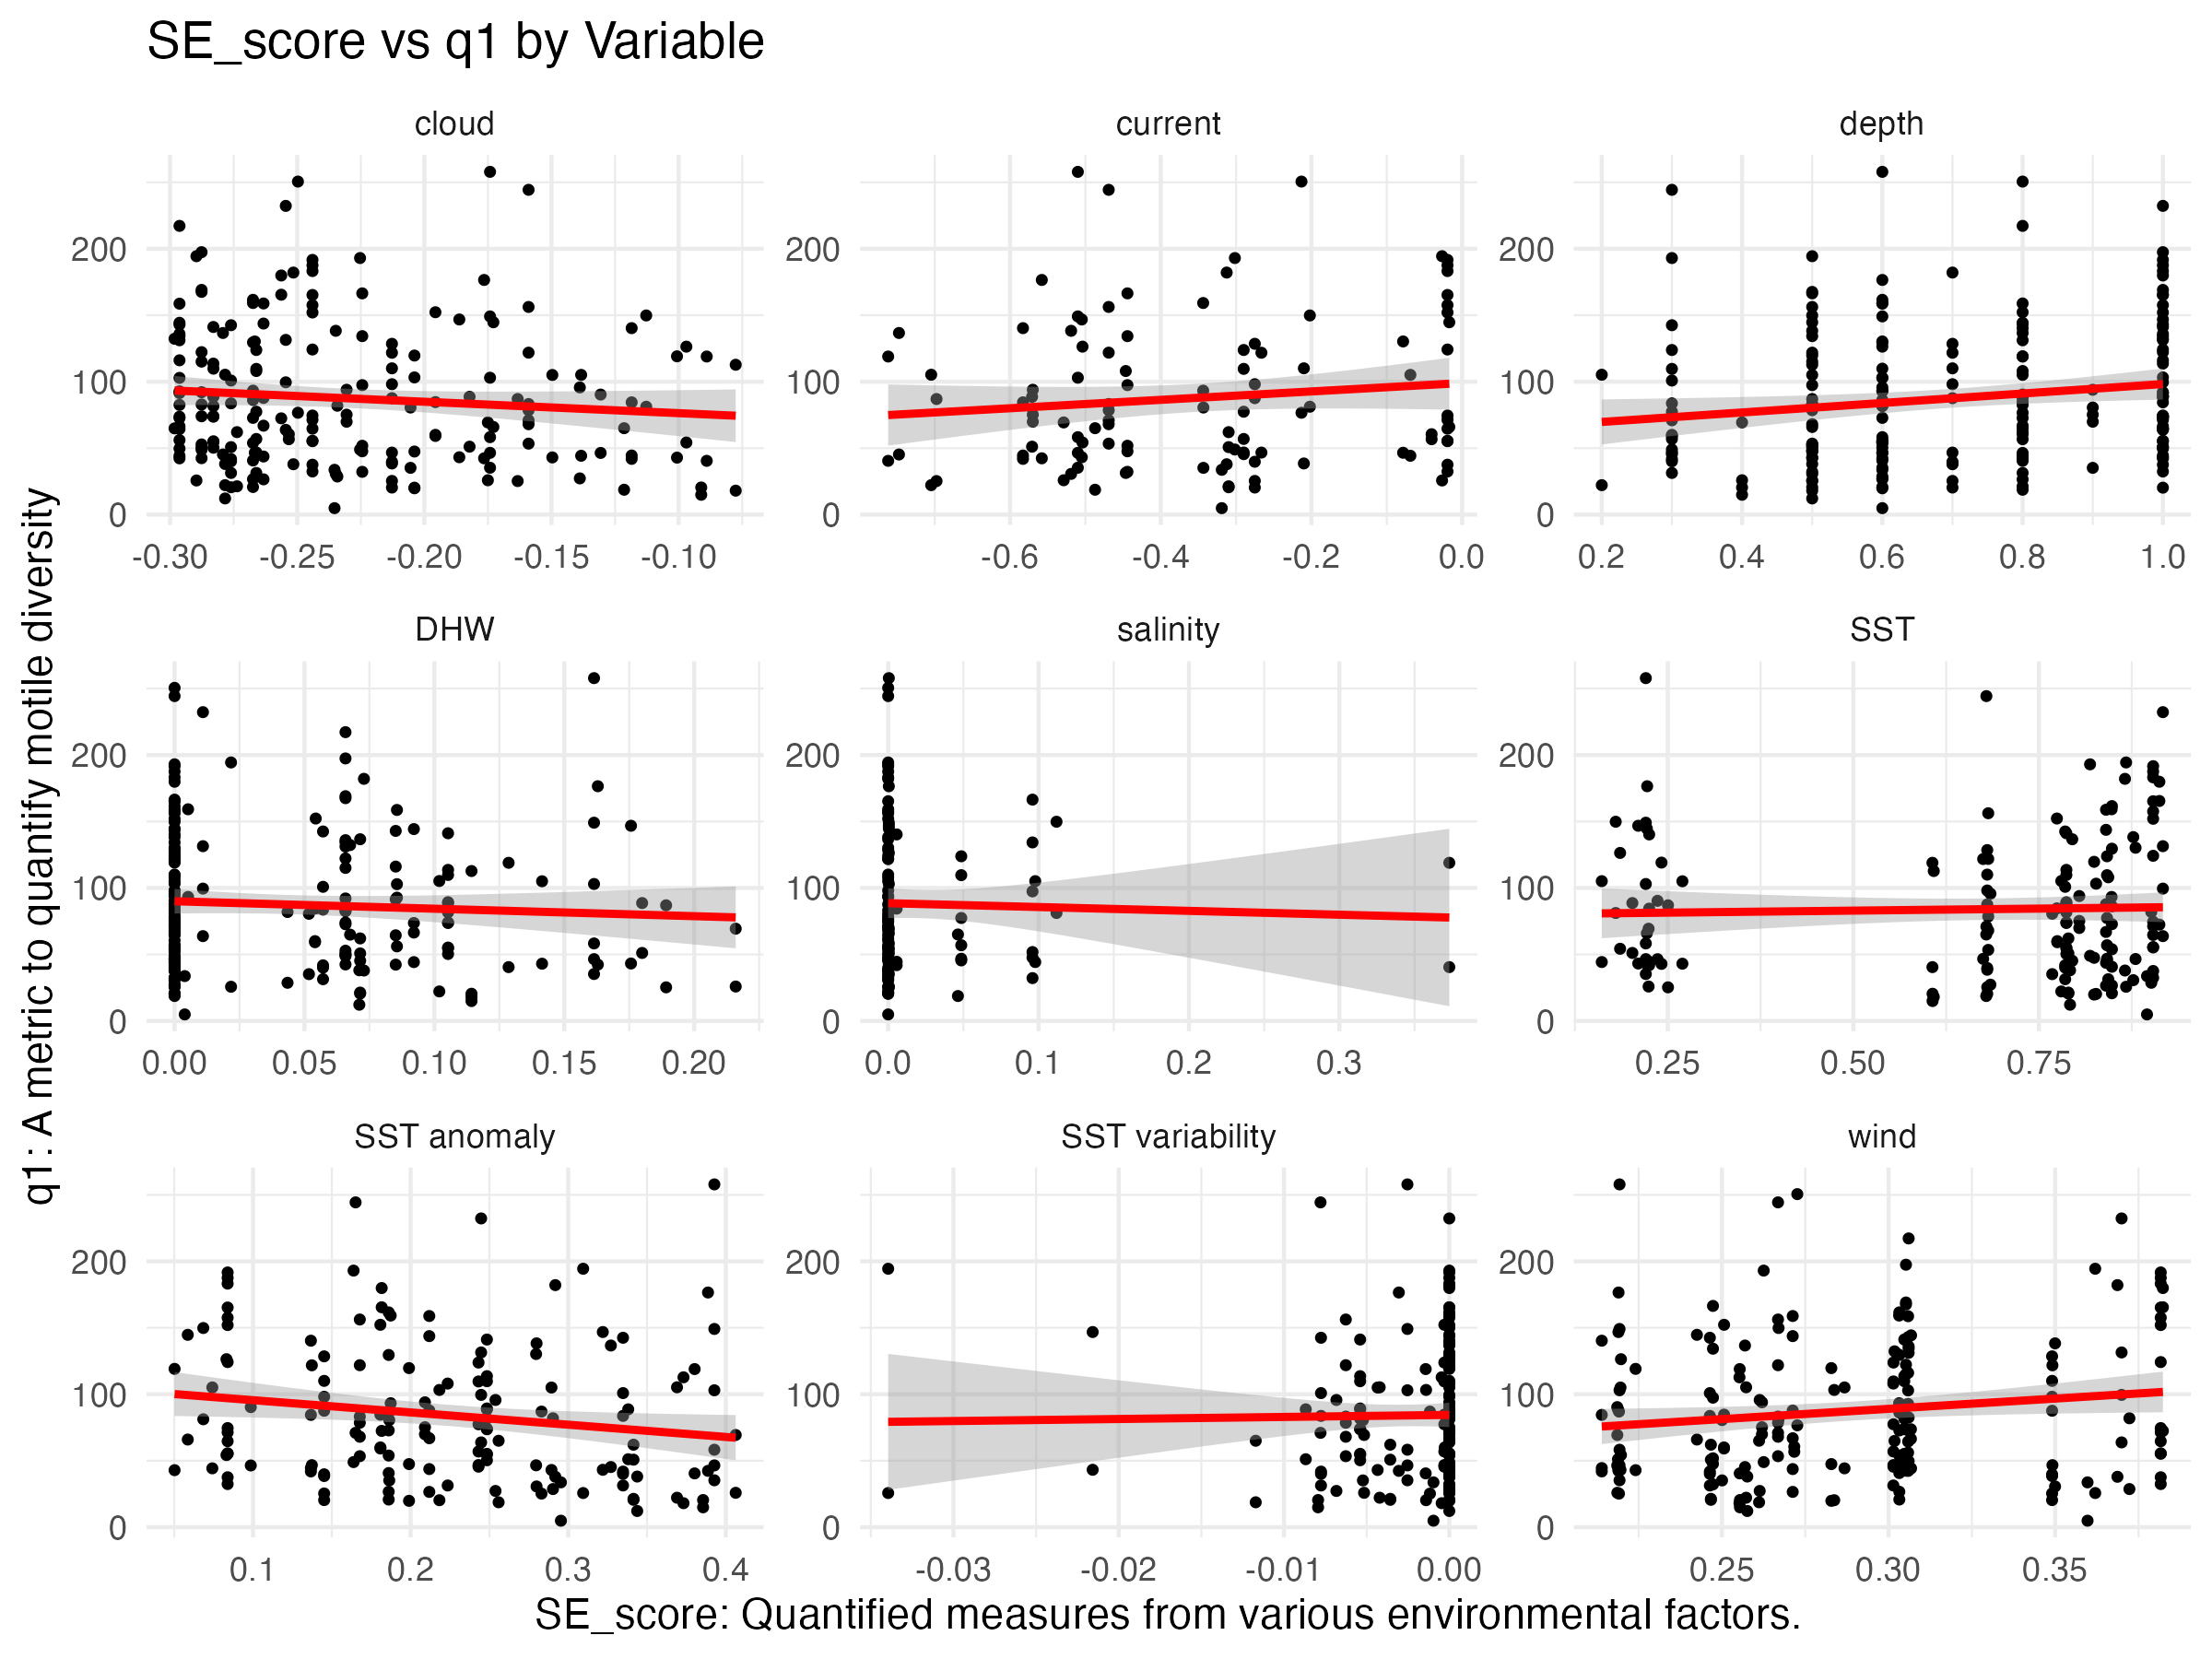
\includegraphics{../plot/se_mean.png}}
    \caption{Linear Model Regression Visualization: Individual marine environmental factor scores vs \texttt{q1}. This figure shows scatter plots of the nine independent variables (wind speed, cloud cover, sea surface temperature, etc.) against the dependent variable \texttt{q1}, along with the linear regression fit lines. Each point represents an observation, the red line indicates the linear regression fit, and the gray shaded area represents the confidence interval.}
    \label{fig:se_mean}
\end{figure}

The visualization of all nine linear regression models reveals that there is no clear linear relationship between any individual marine environmental factors and \(q_1\) (figure 3). Moreover, The X-axis range in each of the nine subplots includes both positive and negative values, reflecting the variability in the environmental factors across different conditions, with positively scored factors being stressors and negatively scored factors being reducers. For example, cloud coverage (cloud) has a negative score, and as the absolute value of this score reaches its maximum, we observe that the distribution range of the diversity index \(q_1\) becomes increasingly broad compared to the zero value. However, not all stressors follow this trend. For instance, in the depth data, we found that the distribution of \(q_1\) is relatively uniform across different depths. In contrast, in the salinity (salinity) data and the variability in Sea Surface Temperature (SST variability), \(q_1\) data are concentrated near the zero value of SST variability. Therefore, a linear description cannot summarize the impact of all environmental factors on \(q_1\).





\begin{figure}[H]
    \centering
    \adjustbox{max width=\linewidth}{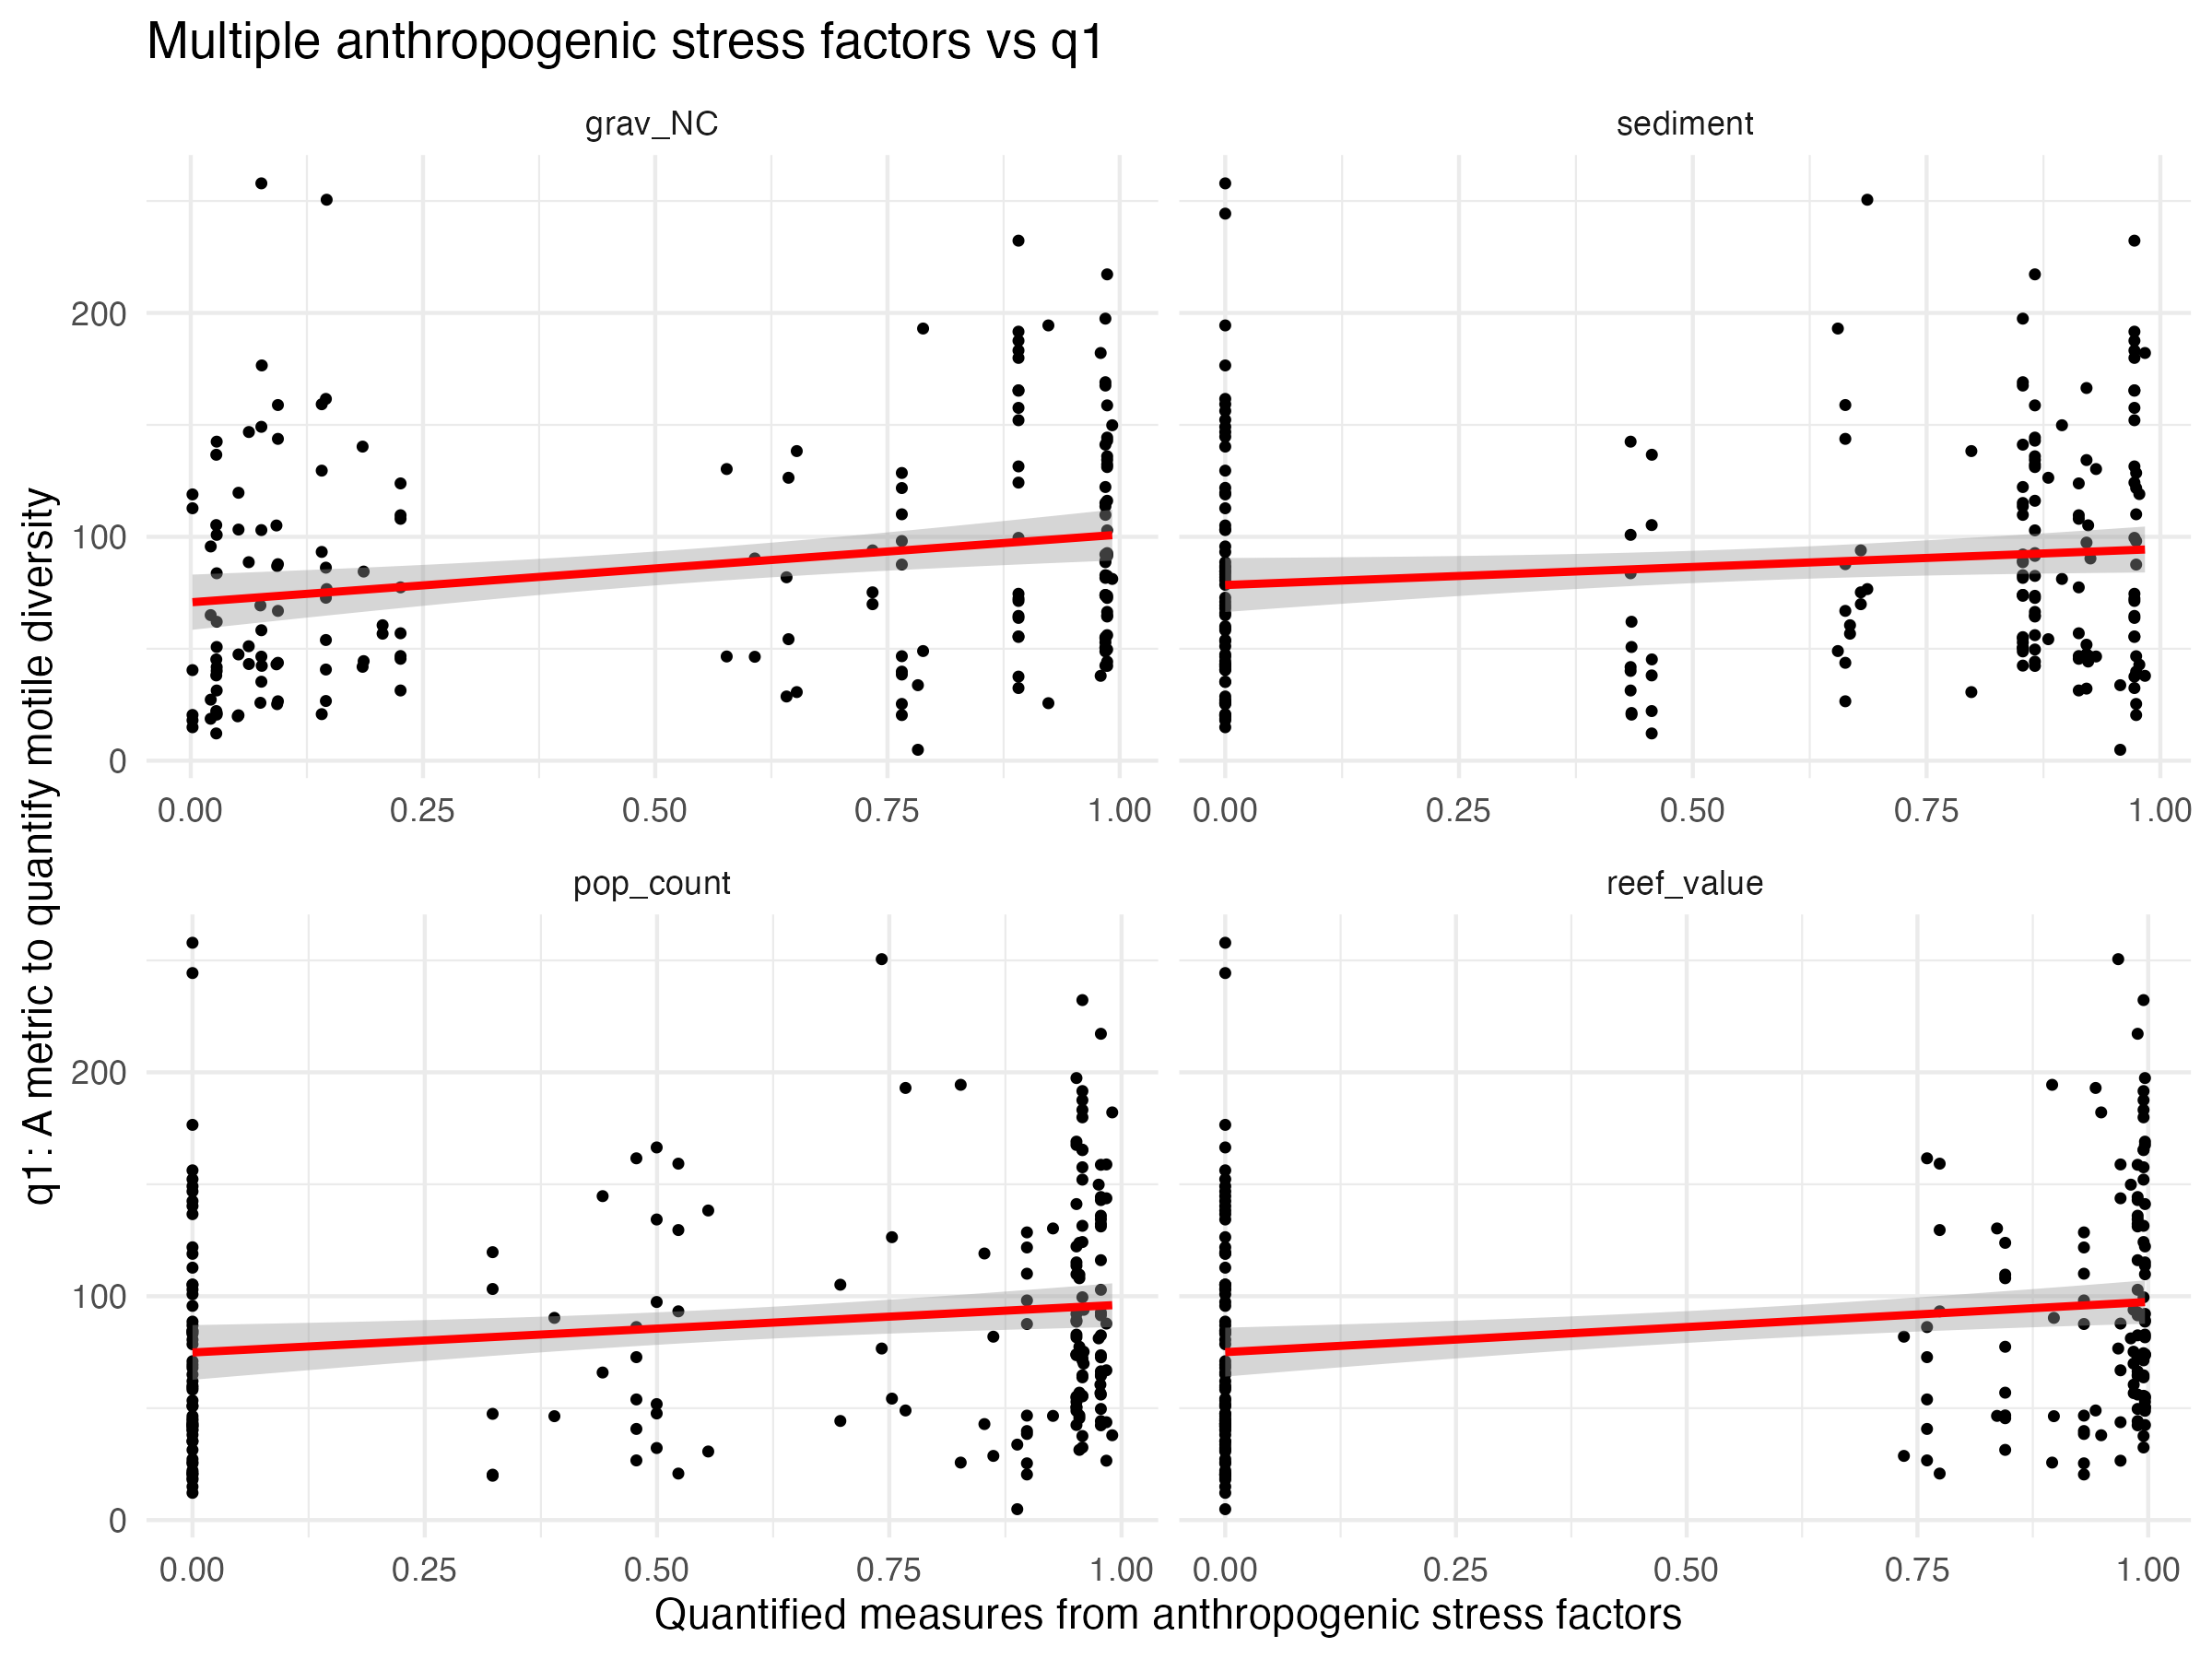
\includegraphics{../plot/all_anthroStress_q1.png}}
    \caption{Linear model regression: individual anthropogenic stressors score vs \texttt{q1}. This graph shows a scatter plot of four independent variables: Fishing(grav\_NC), Sediment, Coastal development(pop\_count) and Tourism(reef\_value) versus the dependent variable \texttt{q1}, along with a linear regression fit line. Each point represents an observation, the red curve indicates the quadratic polynomial regression fit, and the grey shaded area represents the confidence interval.}
\end{figure}


From the linear regression models (figure 4), we can see four individual stressors. The reason for not selecting all six stressors is that the data for Nitrogen (nutrient) and Industrial development (num\_ports) contain a large number of zero values, with most of the data being 0 or 1. Excessive extreme values can lead to inaccurate data analysis, so these two datasets were not analyzed in this study. The figure shows that with the increase in fishing pressure, q1 shows a more obvious linear increase trend, while the other three factors have less obvious effects on q1. The data for the other three stressors (sediment, tourism (reef\_value), and Coastal development (pop\_count)) contain a large number of zero values and show weaker or negligible trends. This suggests that grav\_NC may be a more critical factor affecting q1, while sediment, population count, and reef value have less or more complex effects on q1, requiring further study of these variables.



\begin{figure}[H]
    \centering
    \adjustbox{max width=\linewidth}{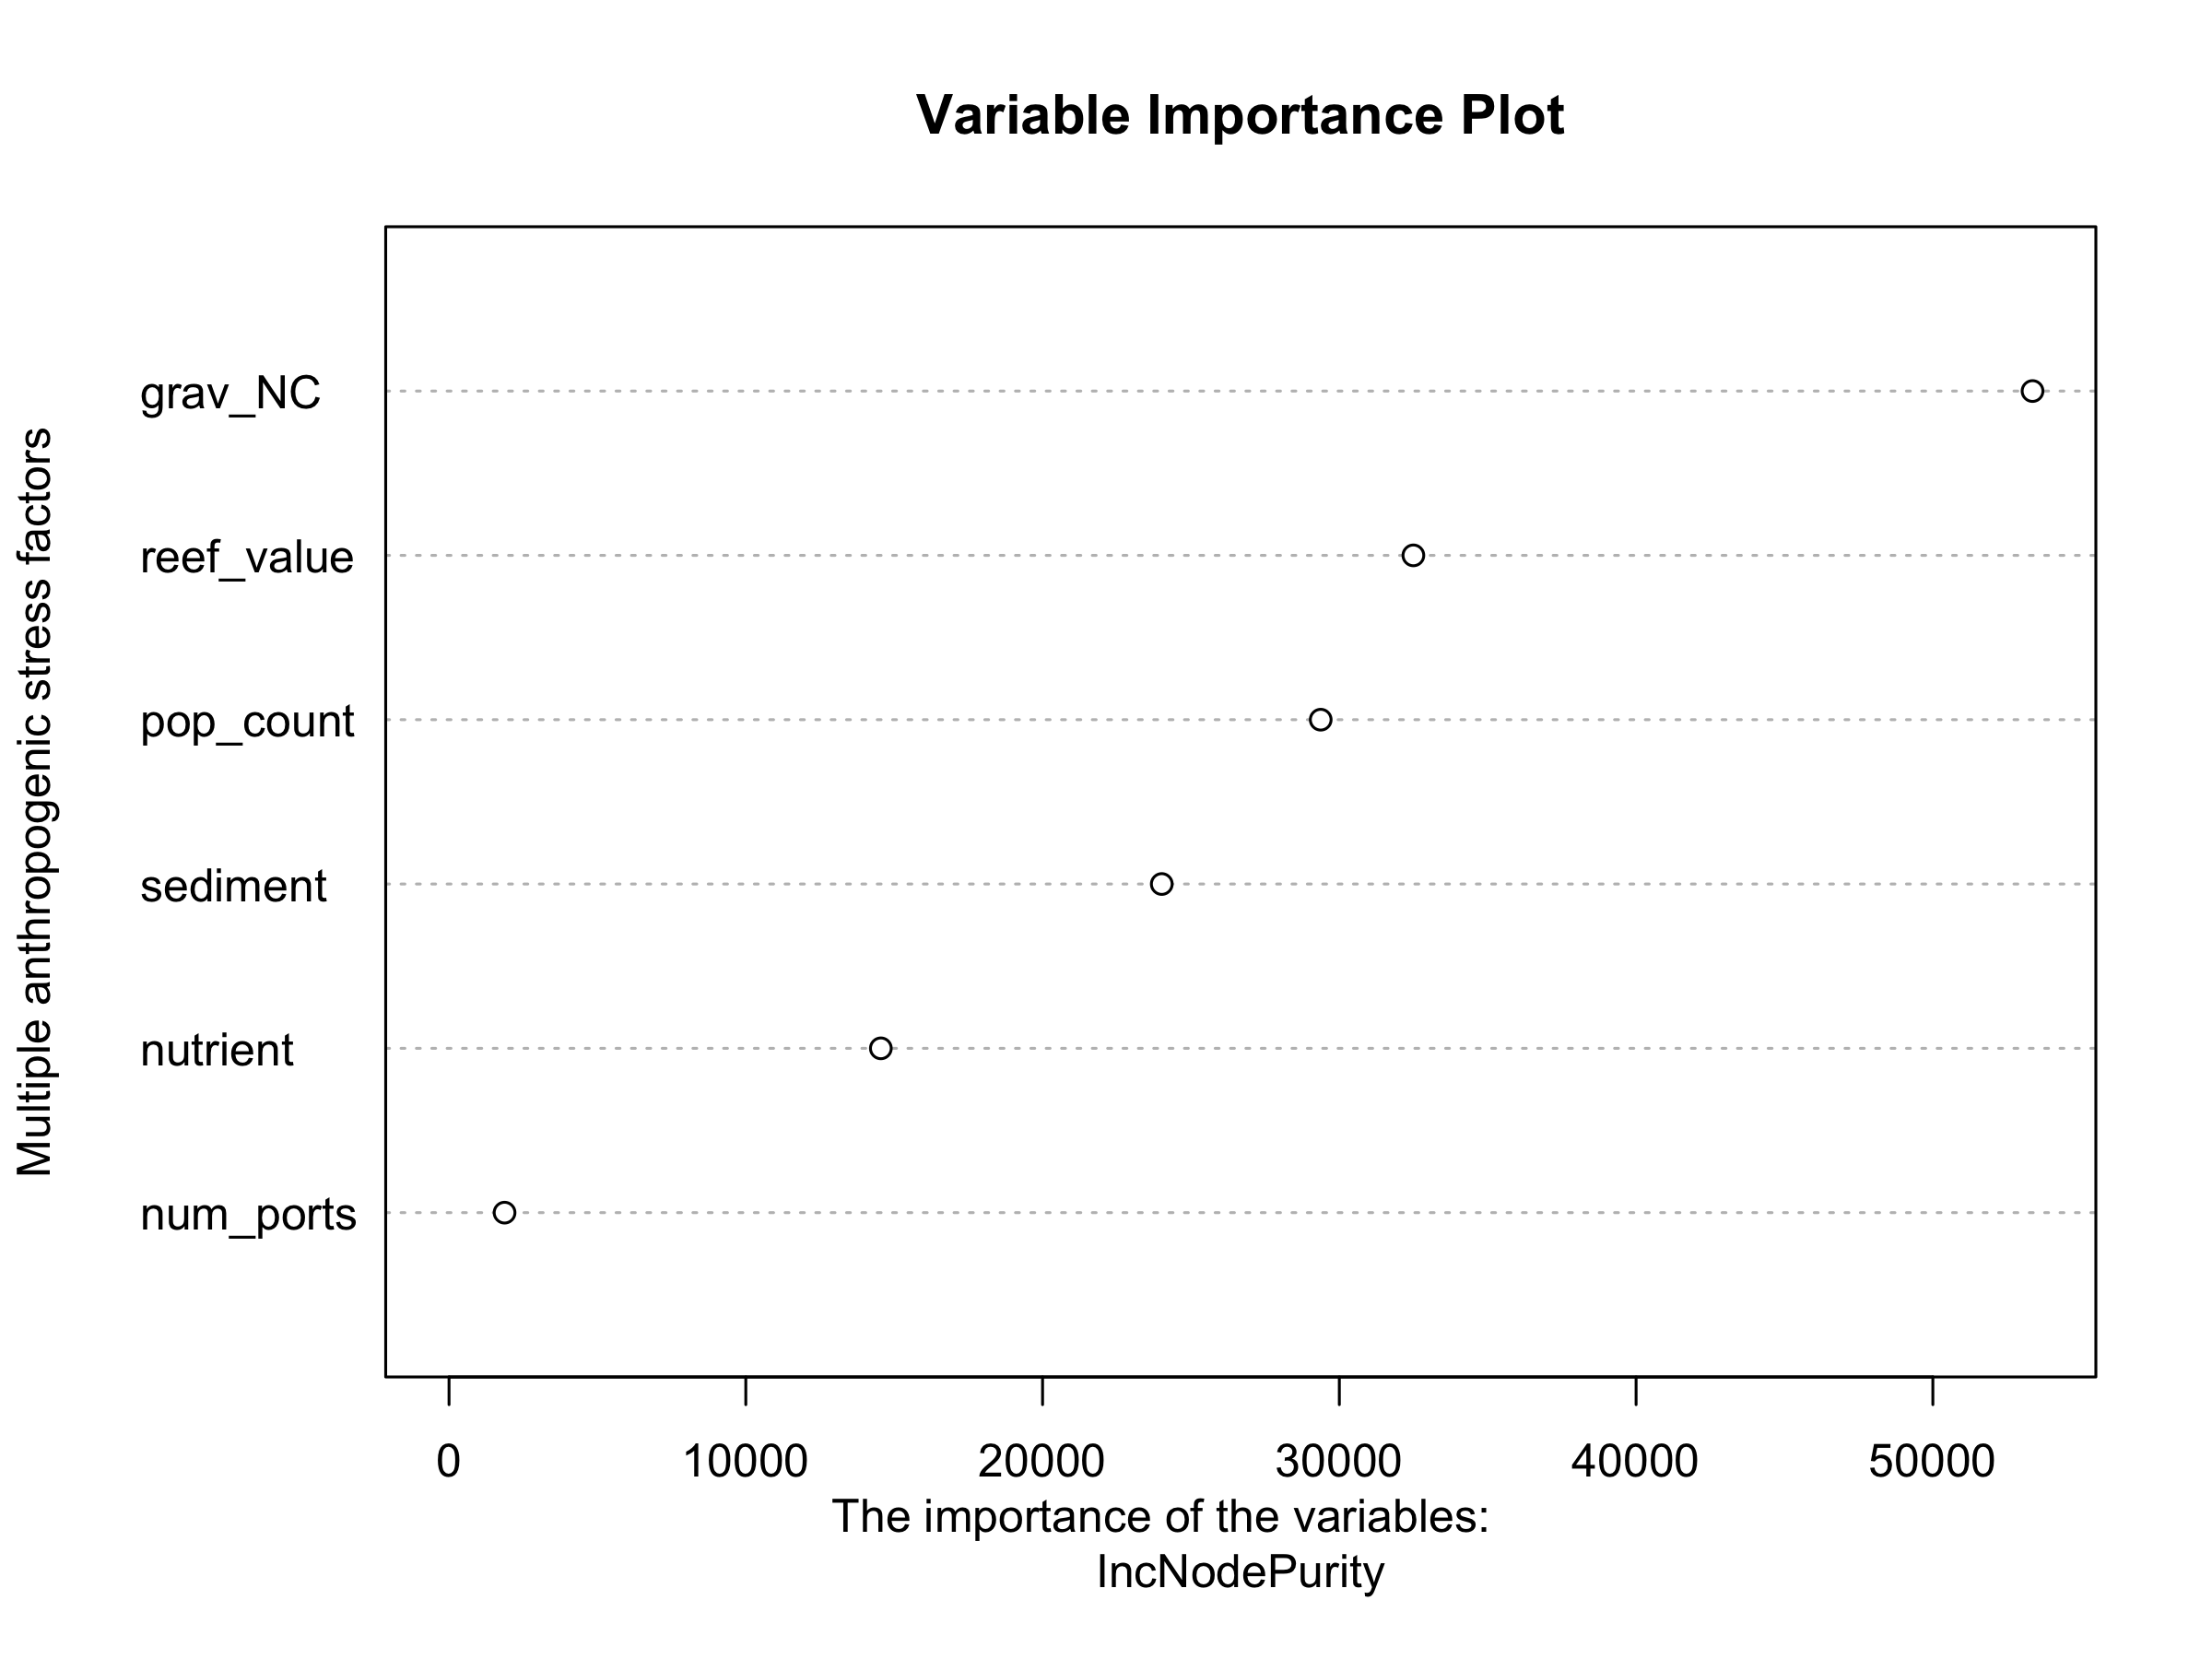
\includegraphics{../plot/RandomF_AS.png}}
    \caption{The importance of various variables in the Random Forest model, The horizontal axis represents the importance metric (IncNodePurity). IncNodePurity is a method for measuring the importance of each variable in a Random Forest model. It evaluates the importance of a variable by calculating the increase in purity brought by each node split (i.e., the reduction in impurity before and after the split). The vertical axis lists different anthropogenic stressors, including fishing (grav\_NC), tourism (reef\_value), coastal development (pop\_count), sediment (sediment), nitrogen (nutrient), and industrial development (num\_ports).}
\end{figure}

To further analyze the impact of different anthropogenic stressors on motile diversity in coral reef systems, we used a Random Forest model to find the extent of these factors' effects on diversity. The results of the variable importance analysis of the Random Forest model meet our requirement (see figure 5). he horizontal axis represents the importance of the variables (IncNodePurity), and the vertical axis lists the six main anthropogenic stressors. We used the entire dataset to train the Random Forest model and generated the variable importance plot. The Random Forest model consists of 500 trees. The results show the importance of six variables, which is the cumulative and average increase in purity brought by a variable when splitting tree nodes, representing the variable's contribution to the model's predictive performance. From the analysis of variable importance generated from a Random Forest model, it is clear that fishing (grav\_NC) contributes the most to the model's prediction, followed by tourism (reef\_value) and coastal development (pop\_count). The importance of sediment (sediment) and nitrogen pollution (nutrient) is relatively low, while industrial development (num\_ports) contributes the least. These results indicate that, under the current model and data, fishing (grav\_NC) is the factor that has the most significant impact on motile diversity in coral reef ecosystems, while industrial development (num\_ports) has the least impact, which can be almost ignored.



% Discussion 
\section{Discussion}
Previous studies have shown that coral reefs undergo erosion due to natural processes, such as weathering and wave action, as well as anthropogenic factors, including climate change and pollution. This degradation of the coral structure affects the complexity and diversity of the reef, in turn leading to significant declines in reef species richness \citep{enochs2012species}. In contrast, in this study we found that comprehensive anthropogenic stressors have a positive impact on motile diversity of coral reef ecosystems. Our finding may be attributed to different geographic locations or methodological approaches. For instance, \citet{enochs2012species} was conducted at various locations in the Caribbean, specifically including the upper Florida Keys. Compared to our research, their study covered a smaller geographic area. In addition, the difference in motile diversity could be due to some individual stressor data used in our study that contains a large number of zero values, which may affect the accuracy of the model results. These zero values could be due to actual ecological phenomena (e.g., the absence of specific stressors in certain areas) or issues during data collection. An excessive number of zero values may make the model insensitive to the impact of certain variables, potentially leading to an underestimation or overestimation of the effects of certain stressors. In this case, we opted to remove excessive non-zero values from the data or to exclude data with a large number of zero values from the analyses, which may improve the accuracy of predictions and the interpretability of the model. 

A variable importance analysis of individual anthropogenic stressors using the Random Forest model shows that fishing (\textit{grav\_NC}) has the greatest impact on \textit{q1} among the six anthropogenic factors, indicating that fishing has a positive effect on motile diversity in coral reef ecosystems. Additionally, the Predator Release Hypothesis proposed by \citet{paine1974intertidal} can almost explain why fishing increases motile diversity in coral reef systems. The reason is that increased fishing activity typically catches large predatory fish and competitively dominant species. The reduction of these species in turn reduces predation and competition for smaller or less competitive species thereby increasing biodiversity in the system \citep{paine1974intertidal}.

Another major threat faced by coral reef ecosystems is marine environmental factors. By monitoring the environmental stress on coral reefs using the RESET tool, we explored its impact on q1 using polynomial regression. We found that when stress appears and continues to increase, the diversity index q1 shows a "U"-shaped trend, first decreasing and then recovering or even increasing. Initially, environmental disturbances (such as typhoons, rising sea temperatures, pollution, etc.) lead to a direct decrease in motile organisms. These disturbances typically cause death, migration, or temporary avoidance, leading to a decline in species numbers. But as the stress continues, the reduction in the abundance of dominant species provides space for the survival of other species, and some species in the coral reef system adapt to the stress, so the number of species gradually recovers after falling to a certain level \citep{graham2006dynamic}. Connell discussed a similar change in his 1978 paper "Diversity in Tropical Rain Forests and Coral Reefs" and proposed the "Intermediate Disturbance Hypothesis": this hypothesis suggests that in the absence of disturbance, dominant species will gradually take over and outcompete weaker species. However, moderate disturbance can prevent any single species from becoming too dominant, thereby maintaining higher species diversity. In coral reef systems, moderate natural disturbances (such as storms of moderate intensity or predation) help prevent certain dominant species from overgrowing, providing habitat space and resources for other species \citep{connell1978diversity}. Meanwhile, a moderate resource supply rate provides sufficient resources to support a diverse community of species \citep{huston1979general}.

The main influencing factors of the marine environment include rising sea and sea surface temperatures, salinity fluctuations, water flow, wind speed intensity, and depth effects \citep{williamson2022monitoring}.  Research by \citet{anthony2011ocean} indicates that the combined effects of ocean acidification and warming exacerbate the negative impacts on coral reefs. For instance, elevated sea temperatures accelerate coral bleaching, while acidification reduces coral calcification capacity, thereby weakening the structural integrity of corals. Under the combined action of these environmental stress factors, we further studied the changes in motile diversity in coral reef ecosystems. The predicted values of RESET\_score did not have a significant impact on the motile diversity in coral reef systems in the lm model, indicating that marine environmental factors do not continuously cause a decrease or increase in species diversity. Moreover, RESET\_score is a multi-indicator environmental stress exposure index formed by integrating individual stress factors such as sea surface temperature, wind speed intensity, and depth \citep{williamson2022monitoring}. However, the results of the linear regression model of individual marine environmental factors with q1 (Figure~\ref{fig:se_mean}) did not show significant linear relationships. In these individual environmental factors, \citet{williamson2022monitoring} identifies some as stressors (Sea Surface Temperature, Degree Heating Weeks, etc.), while others are classified as reducers (Cloud Cover, Current, etc.). Stressors are the primary drivers that negatively impact coral reefs, often leading to deterioration in coral health. On the other hand, reducers are factors that help enhance the resilience of coral reefs by mitigating or offsetting the negative effects of stressors. Similarly, \citet{zhu2022impact} also highlights that the rise in ocean temperatures leads to widespread coral bleaching, while coastal upwelling areas, which bring cooler water, may help alleviate this thermal stress \citep{zhu2022impact}. In addition, the results of this study also show that there are obvious differences in the distribution of various marine environmental stressors, and there is no linear relationship between them and q1. This implies that more models are needed to explain these data. Therefore, assessing the impact of specific environmental conditions on motile diversity in coral reef systems through linear models may be challenging and may not capture the full complexity of these interactions.

Coral reef ecosystems are subject to the combined effects of multiple stressors, which may interact in complex ways. This study analyzed the joint effects of two major stressor cumulative scores (marine environmental stressors and anthropogenic stressors). However, when analyzing these factors individually, the cascading effects between pairs or multiple factors might be overlooked, which could lead to an oversimplification of certain phenomena and fail to fully reflect the true state of the ecosystem. The cascading effects are crucial when studying the impacts on coral reef ecosystems. The degradation of coral reefs leads to fish losing their habitat and food sources, which in turn results in a decline in fish populations. This decline not only affects the balance of the ecosystem but also impacts fisheries \citep{hoegh2011impact}. Future research could focus on more detailed studies of cascading effects, looking at how changes in one part of the ecosystem might lead to broader impacts on other areas. Such research could also explore the temporal and spatial scales at which these cascading effects operate,  thereby gaining deeper insights into the impact on species diversity within coral reef ecosystems under constantly changing environmental conditions.


% conclusion 
\section{conclusion}

Our study demonstrates that motile diversity within marine coral reef ecosystems is influenced by both anthropogenic pressures and natural oceanic environmental factors. The effects of these pressures on diversity are complex. Based on our current data analyses, we found with a linear model that the overall anthropogenic pressure score is positively correlated with motile diversity. However, the presence of numerous zero values in some individual anthropogenic pressure data might contribute to inaccuracies in the analysis. In this case, we utilized a random forest model to visualize the importance of different variables, allowing us to explore the extent to which various anthropogenic pressure factors influence diversity. Due to the complex interactions and variability of oceanic environmental pressures, we were unable to establish a straightforward linear relationship between these factors and motile diversity. Nevertheless, using a polynomial regression model, we identified a nonlinear relationship between motile diversity and the overall environmental score (RESET score), which exhibits a "U-shaped" trend. We did not find a significant model to explain the relationship between motile diversity and individual oceanic environmental factors. These results reveal the complex responses of motile biodiversity in coral reef ecosystems to anthropogenic and natural environmental pressures. Within certain limits, anthropogenic pressures and natural environmental pressures may influence species distribution and diversity by altering the structure of the ecosystem. Looking forward, the collection of more detailed and accurate data will be key to advancing research, enabling a more comprehensive understanding of the impact of various stressors on species diversity within marine coral reef ecosystems. Additionally, integrating data across different ecological levels, such as species, communities, and ecosystem functions, will help reveal the multiple effects that these stressors have on biodiversity. Future research should also consider developing and applying more complex models to explore the interactions and cumulative effects among stressors, thereby providing a stronger scientific basis for ecosystem conservation and management.

\section{Data and Code Availability}

All data and codes in this project are available at:
\url{https://github.com/BlackMamba4ever/CMEECourseWork/tree/master/Final\_Project}. For further information of code and data, please see README.md.

% References
\bibliographystyle{apalike}
\bibliography{ref} % Replace with your actual .bib file
\end{document}
